\documentclass[a4paper,11pt,fleqn]{article}%fleqn pour aligner les equations à gauche
\usepackage{../../Styles/Cours}

\newcommand{\chnum}{Chapitre 17}
\newcommand{\chtitle}{Casque anti-bruit actif}
\newcommand{\dtype}{Activité}

\begin{document}
\maketitle
En matière de protection auditive, il existe des protections passives et des protections actives. Les premières ne constituent qu'une barière physique pour la protection du son : mousse, cire ou casque complet. Les secondes ont besoin de batteries pour fonctionner. Elles intègrent un circuit électronique comportant un haut parleur et un micro et un software permettant par exemple de bloquer le bruit d'un marteau-piqueur tout en laissant une voix humaine audible.\\
\textbf{Comment fonctionne un casque d'atténuation active ?}

\begin{figure}[h!]
    \caption{Fonctionnement du casque antibruit actif}
    L'air oscille sous l'impulsion des ondes sonores, c'est-à-dire que sa pression augmente puis diminue régulièrement. Dans le casque actif, on crée un second signal de telle sorte qu'une dépression de l'air due au bruit soit compensée par une compression et réciproquement. Ainsi pour l'oreille, la variation de pression est alors quasiment nulle, le son a été supprimé.\\
    \begin{minipage}{.4\linewidth}
        Le casque actif doit ainsi comporter, entre autres, un microphone pour capter le bruit, un composant électronique pour analyser le bruit et un haut parleur pour émettre le signal correcteur.
    \end{minipage}
    \begin{minipage}{.58\linewidth}
        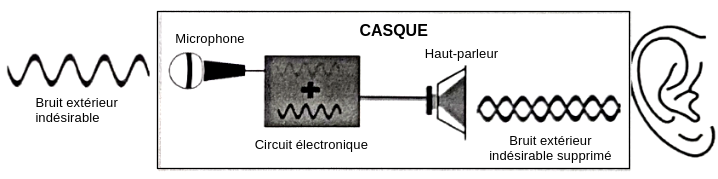
\includegraphics[width=\linewidth]{Ressources/TSPE_C17_Act2_Fig1.png}
    \end{minipage}
    \label{doc1}
\end{figure}

\begin{figure}[h!]
    \begin{minipage}{.7\linewidth}
        \caption{Extrait d'un programme Python}
    \begin{lstlisting}[language=Python]
        import numpy as np
        import matplotlib.pyplot as plt

        #Creation d'une variable temps, t, prenant 100 valeurs entre 0 et 0.1 sec
        t = np.linspace(0,0.1,100)
        # Creation de la grandeur amplitude
        A1=float(input('Amplitude du dignal 1 : A1 = '))
        # On fixe la frequence du signal a 50 Hz
        f = 50
        # On fixe le dephasage phi a pi
        phi=np.pi

        ####################################
        # Definition d'une fonction sinusoidale y1 d'apres les parametres au dessus
        y1=A1*np.cos(2*pi*f*t+phi)
    \end{lstlisting}
    \label{doc2}
    \end{minipage}\hspace{.02\linewidth}
    \begin{minipage}{.28\linewidth}
        \caption{Mathématiques}
        L'expression mathématique d'un signal sinusoïdal est : $$y(t)=A \cdot \cos(2\pi \cdot f \cdot t + \phi) $$
        Avec $A$, son amplitude, $f$ sa fréquence et $\phi$ sa phase à l'origine.
    \end{minipage}
\end{figure}

\begin{enumerate}
    \item Expliquer brièvement ce que permet de réaliser le code décrit dans le Document \ref{doc2}.
    \item Influence du déphasage entre deux courbes sinusoïdales.\\
    Ouvrir le programme TSPE\_C17\_Casque.py avec EduPython.
    \begin{enumerate}
        \item Ligne 18, compléter avec une ligne permettant de créer une fonction sinusoïdale $y_2$ ayant la même amplitude que $y_1$ mais déphasée de $\dfrac{\pi}{2}$ par rapport à $y_1$
        \item Lancer le programme en choisissant une amplitude $A1$ de valeur 1. Faire vérifier votre graphique.
        \item Faire varier le déphasage de $y_2$, successivement pour des valeurs de $\pi$, $\dfrac{3\pi}{2}$ puis $2\pi$.
    \end{enumerate}
    \item Modélisation du fonctionnement du casque antibruit.
    \begin{enumerate}
        \item D'après le Document \ref{doc1} et les résultats de la question 2, quel déphasage par rapprot au bruit extérieur doit avoir l'onde sonore créée par le casque ?
        \item Ligne 21, transformer la variable $y_3$ pour la définir comme la somme de $y_1$ et $y_2$.
        \item Lancer le  programme avec différentes valeurs d'amplitude. Que constatez-vous ? Définir les conditions nécessaires pour atteindre l'objectif.
    \end{enumerate}
\end{enumerate}

\end{document}

